% The cross product: a cube U in X and a cube V in Y give a product cube U×V
% in the product space X×Y.
% Source: book/tex/homology/cup-product.tex (§ Cross product).
\documentclass[border=2mm]{standalone}
\usepackage{tikz}
\usetikzlibrary{arrows.meta}
\begin{document}
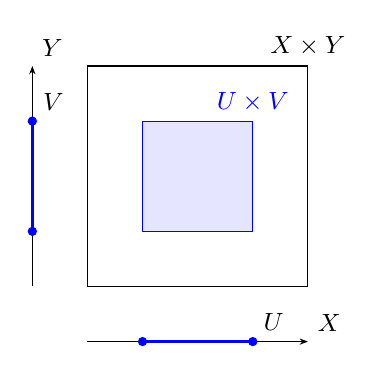
\begin{tikzpicture}[scale=1.4, >={Stealth[length=3pt]}, every node/.style={font=\small}]
  \draw[->] (0.5,0) -- (2.5,0) node[above right] {$X$};
  \draw[->] (0,0.5) -- (0,2.5) node[above right] {$Y$};
  \draw[blue, very thick] (1,0) -- (2,0) node[above right, black] {$U$};
  \fill[blue] (1,0) circle (1.2pt); \fill[blue] (2,0) circle (1.2pt);
  \draw[blue, very thick] (0,1) -- (0,2) node[above right, black] {$V$};
  \fill[blue] (0,1) circle (1.2pt); \fill[blue] (0,2) circle (1.2pt);
  \fill[blue, opacity=0.1] (1,1) rectangle (2,2);
  \draw[blue] (1,1) rectangle (2,2);
  \node[blue, above] at (2,2) {$U \times V$};
  \draw (0.5,0.5) rectangle (2.5,2.5);
  \node[above] at (2.5,2.5) {$X \times Y$};
\end{tikzpicture}
\end{document}
